\documentclass{article}

\usepackage[utf8]{inputenc}

% Packages
\usepackage{amsmath,amssymb}
\usepackage{bm}% boldmath
\usepackage{listings} % Code block (source code) \begin{lstlisting} 
\usepackage{natbib}
\usepackage{graphicx}
\usepackage{lmodern}
\usepackage[usenames,dvipsnames,svgnames,table]{xcolor}
\usepackage[textwidth=16cm,textheight=23cm]{geometry}

%\usepackage{inconsolata} % New monospace font

% URL
\usepackage{url}
\usepackage[colorlinks=true, a4paper=true, pdfstartview=FitV, linkcolor=blue, citecolor=blue, urlcolor=blue]{hyperref}

% Figures
\usepackage[font=small, labelfont=bf]{caption}
\usepackage{subfig} % Subfigures. Uses \subfloat[captions text]{figure}

% Tables
\usepackage{booktabs}   % Allows the use of \toprule, \midrule and \bottomrule in tables for horizontal lines
\newcommand{\ra}[1]{\renewcommand{\arraystretch}{#1}} % spaces in tables

% Itemize
\usepackage{enumitem}

% Commands
%\newcommand{\code}[1]{\texttt{#1}} % \code{inline code}
\newcommand{\code}[1]{{\small\ttfamily #1}} % \code{inline code}
\newcommand{\expval}[1]{\langle #1 \rangle} %
\renewcommand{\theequation}{\arabic{section}.\arabic{equation}} % Book format equation
\renewcommand{\thefigure}{\arabic{section}.\arabic{figure}} % Book format figure
\renewcommand{\vec}[1]{{\bf #1}} % Lars likes this better than arrow

% Set page attribution
\setlength{\parindent}{0pt}


% PSTRICKS
\usepackage{pstricks,pst-node,pst-tree} % includes graph additions
\usepackage{pst-pdf} % Compiles the pictures
\usepackage{pst-node}
\usepackage{pst-plot}
\usepackage{pst-3dplot}
%\usepackage{pstricks-add,babel}




\lstset{
language=Python,                        % Code langugage
commentstyle=\color{gray},              % Comments font
basicstyle=\small\ttfamily,             % Code font, Examples: \footnotesize, \ttfamily
keywordstyle=\bfseries\color{blue},
stringstyle=\color{orange},
numbers=left,                           % Line nums position
numberstyle=\tiny,                      % Line-numbers fonts
stepnumber=1,                           % Step between two line-numbers
numbersep=5pt,                          % How far are line-numbers from code
frame=none,                             % A frame around the code
tabsize=4,                              % Default tab size
captionpos=b,                           % Caption-position = bottom
breaklines=true,                        % Automatic line breaking?
breakatwhitespace=false,                % Automatic breaks only at whitespace?
showspaces=false,                       % Dont make spaces visible
showstringspaces=false,                 % Dont make spaces visible in strings
showtabs=false,                         % Dont make tabls visible
belowskip=8pt,
morekeywords={range, xrange},
% backgroundcolor=\color{yellow}
% emph={[2]root,base}
% morekeywords={one,two,three,four,five,six,seven,eight,
}


%commentstyle=\color{gray},              % Comments font
%basicstyle=\small,                      % Code font, Examples: \footnotesize, \ttfamily



%basicstyle=\footnotesize\ttfamily,
%keywordstyle=\bfseries\color{green!40!black},
%commentstyle=\itshape\color{purple!40!black},
%identifierstyle=\color{blue},
%stringstyle=\color{orange},







% ***************************************************
% HEADER INFORMATION

\title{Exercise 1}
\author{Molecular Statistics, Week 1}
\date{2014}

% ***************************************************

\begin{document}


% ***************************************************
% BEGIN DOCUMENT
% ***************************************************

\maketitle

\section{Introduction}

This is the first exercise in the course Molecular Statistics. The exercises
throughout the course are split into two parts. The first part is a general
introduction to new concepts and programming techniques. The second part is to use
Python to simulate physical systems.\\

The curriculum can be found here 
\href{http://pymbook.readthedocs.org/en/latest/}{pymbook.readthedocs.org/en/latest},
which will contain all the concepts.
Additional information can be gained by using the very powerful tool called "Google".
For the first week, read the following chapters;

\begin{itemize}
    \item \href{http://pymbook.readthedocs.org/en/latest/thebeginning.html}{Introduction}
    \item \href{http://pymbook.readthedocs.org/en/latest/variablesanddatatypes.html}{variables and datatypes}
    \item \href{http://pymbook.readthedocs.org/en/latest/operatorsexpressions.html}{operators and Expressions}
    \item \href{http://pymbook.readthedocs.org/en/latest/ifelse.html}{If Else}
    \item \href{http://pymbook.readthedocs.org/en/latest/looping.html}{Looping}
\end{itemize}


\section{Python}

To execute a program written in Python, we save a file with the extension
'.py' and run it via the terminal using the following syntax:

\begin{lstlisting}
python example_program.py
\end{lstlisting}

Now, let's start by using Python as a calculator.
Remember to print the result of your calculation using the \code{print} statement.
We encourage you to have some sort of logical file system, saving all the exercises in
different files and folders so you can find it again when needed.

\begin{enumerate}
  \item Execute the following statements. Does it behave like your regular
    calculator? If anything unusual happens try and explain why.
    {\em Hint}; what is the difference between {\bf integer} and {\bf float}?

    \begin{centering}
      \code{5+9, 5-9, 5*9, 5/9, 5+2*9, 5.0+2.0*9.0, 5.0/9 5**2,
        5\%2}
    \end{centering}
\end{enumerate}

Since manually entering numbers really does us no good, we might as well use a
calculator. Instead, we want to utilize what programming languages can provide,
namely storage of values in what is known as {\bf variables}. Variables can store
anything that you can think of, i.e. numbers, strings, lists of numbers and so
forth. Variables are assigned values by specifying a variable name and a value, e.g.

\begin{lstlisting}
my_first_variable = 5.0
\end{lstlisting}

where a variable named \code{my\_first\_variable} has been assigned the value
of $5.0$.
Some restrictions apply for variable names (must start with a letter, can't have names of
in-build functions etc.), but otherwise we are not restricted in the naming. We encourage you to give
them useful names, such as \code{no\_particles} for representing number of
particles. That way you can more easily remember what values are stored in the variable
and it makes the code more readable for others.\\

Since a variable can contain anything, a very useful function is \code{type(arg)},
where \code{arg} is a variable. This function will return the type of value stored
in the variable.

\begin{enumerate}
  \setcounter{enumi}{1}
  \item Execute the same statements from task 1, but using variables to store
    the values and results. Print the results.
  \item Use \code{type} to print out the type of the variables used.
\end{enumerate}

Usually when working with a program we work with a range of numbers
that we need to manipulate, and for this it is fairly useful to create a Python {\bf list}
of numbers.
A list is defined with the same syntax as a float variable;

\begin{lstlisting}
simple_list = []
\end{lstlisting}

The above code creates an empty list named \code{simple\_list}.
Even though the list is empty we can still print
the content of the variable (try it).
If you want to add an element to the list you can
append it using \code{list\_name.append(arg)} where \code{arg} is the element to append the list.

For example if you want to append 2.0 to a list you write;

\begin{lstlisting}
simple_list.append(2.0)
\end{lstlisting}

\begin{enumerate}
  \setcounter{enumi}{3}
  \item Create an empty list.
    Print the empty list.
    Append a number and print it again.
    What changed in the output?

  \item Print the type of the variable.

  \item Add the following numbers to the list: -1.0, 1.5, 2.0, -2.0, -3.0, 3.0 and
    print the content of the variable again.
\end{enumerate}


Different variables have different attributes, which are called {\em methods}.
These methods are executed using 'dot'.
For instance,
the variable of type list has the method \code{sort()},
which can be called as follows;

\begin{lstlisting}
simple_list.sort()
\end{lstlisting}

For a list of floats, this results in the items of the list being sorted by value.\\

Another way of populating a list with numbers is to do it directly when
we create the list.
This is done almost the same way as when we created the empty list, except we
provide the initial content right away. E.g.

\begin{lstlisting}
another_list = [1.0, 2.0, 3.0, 4.0, -2.0, -4.5, -1.0]
\end{lstlisting}


\begin{enumerate}
  \setcounter{enumi}{6}
  \item Define \code{another\_list} and repeat task 6.

  \item Print the list. Sort the list. Print the sorted list.
  Does it provide the correct result?

  \item Print \code{another\_list} in reverse sorted order.
    Use Google to find out how.\footnote{Using Google is
    by far the most important tool as a programmer.}
\end{enumerate}

% >>> L = [0,10,20,40]
% >>> L.reverse()

We've now seen that python lists can be created in various ways and even be
sorted, but it is quite tedious to enter all data manually. Especially if
there is a lot of it.
Luckily, Python provides us with the means to construct
lists using other approaches.
The \code{range()} command is one of them and is probably the
command that you will spend the most time with during this course.

\begin{enumerate}
  \setcounter{enumi}{9}
  \item Write the following commands in the python shell and explain the results
    before moving on.

    {\em Hint:} use the type command to get the data type of the commands,
    i.e. \code{type(range(10))}

\begin{lstlisting}
print range(10)
print range(3, 10)
print range(-3, 10, 4)
\end{lstlisting}

  \item Understand how the range function works.
\end{enumerate}


If we want to access the i'th element in a list
we use square brackets. To print the second element
in the list from above you write;

\begin{lstlisting}
print another_list[1]
\end{lstlisting}

Notice that we wrote 1 and not 2. This was not a typo!
This is because the list index starts at 0 and not 1.\\

To get the length of a list you use the function \code{len(arg)}
where \code{arg} is the variable with the list.
If you want the length of our example list, the syntax is

\begin{lstlisting}
print len(another_list)
\end{lstlisting}


\begin{enumerate}
  \setcounter{enumi}{11}
  \item Initialize the following list and test your knowledge about
    lists with the following print-statements.
    Describe the result of every print-statement. Test your
    understanding of lists by guessing what the output will be before
    you run it. 
    {\em Hint;} one of the lines will give an error. Why?

\begin{lstlisting}
q_list=[45, 23, 56, 34, 76, 50]

print q_list[3]
print q_list[0]
print q_list[-1]
print q_list[len(q_list)]
print q_list[len(q_list)-1]
\end{lstlisting}

  \item What is the index of the first item in a list? What is the index of
    the last item?

\end{enumerate}

Creating lists from lists. Say that we have a list \code{x\_list}
and we want to create $y$ values as a function of these $x$ values.
To do this we want to iterate over the elements of \code{x\_list} to create the new list.
This is where we want to use {\em for-loops}.
Let's jump straight into the syntax. Say that we already
have defined a variable containing the $x$-values, \code{x\_list},
then \code{y\_list} is created as,

\begin{lstlisting}
y_list = []
for x in x_list:
    y = x**2
    y_list.append(y)
\end{lstlisting}

First we initialize a new list,
then we fill in $y$ values by iterating over
all $x$ values in \code{x\_list}.
As you might have guessed the above code is equivalent to 
the function $f(x) = x^2$.\\

\begin{enumerate}
  \setcounter{enumi}{13}
  \item Create a list of $x$ values from -5 to 5 (both included). Use this list
    to calculate values for another list, with the function $f(x) = -6x^2 + 6x$.
    Print the result.

\end{enumerate}

Another one-line way of working with lists is the following syntax;

\begin{lstlisting}
  y_list = [x**2 for x in x_list]
\end{lstlisting}

which does exactly the same as the above example\footnote{This method is
called ``list comprehension''. Knowing what methods are called makes
it easier to get help from Google when you get stuck. }.

\begin{enumerate}
  \setcounter{enumi}{14}
  \item Repeat exercise 14, but using the shorthand way of creating lists.
\end{enumerate}

What if we want to use math functions (or other modules)?
We can import them! This is always done in the top of the
python file using the syntax;

\begin{lstlisting}
import math
\end{lstlisting}

The math module has a lot of useful mathematical functions like \code{sin},
\code{cos} and \code{exp}. When the math package has been imported it is used
in the following way;

\begin{lstlisting}
print math.cos(180.0)
print math.exp(180.0)
\end{lstlisting}

\begin{enumerate}
  \setcounter{enumi}{15}
  \item Create a list of $x$ values from -5 to 5 (both included).
    Calculate sine values, $f(x) = \sin{x}$ using the math module,
    for the $x$-list.
    Print the result.
  \item Use the matplotlib-manual (found on the website) to save plots of 
    task 14 and 16.
\end{enumerate}


\newpage
\section{Non-Interacting particles}

The goal of today's simulation is to initialize particles with random
coordinates and random velocities confined in a 2 dimensional box,
and propagate the particle positions in time.\\

The code below is your starting point for today's exercise.

\begin{lstlisting}
# Import pyplot and a function to create random numbers
import random
import matplotlib.pyplot as plt

# initialize some variables
n_particles = 100
n_steps = 1
dt = 0.01

# create the x- and y-coordinates
pos_x = [random.random() for i in range(n_particles)]
pos_y = [random.random() for i in range(n_particles)]

# plot the x- and y-coordinates in a figure.
plt.plot(pos_x, pos_y, 'ro')
plt.axis((-1, 1, -1, 1))
plt.savefig('coordinates_start.png')

\end{lstlisting}

As you can see, a lot of variables have been declared such as
\code{n\_particles} which
is the number of particles that we want to generate and simulate.
\code{n\_steps} is
the number of steps we want to take in the simulation
and \code{dt} controls how large a time-step we will be taking.
Lastly we have defined the
$x$- coordinates and
$y$-coordinates for
\code{n\_particles} random particles using list-comprehensions.

\begin{enumerate}
  \item Inspect and understand all lines in the above code.
    Line by line, explain what the code does.
    You should print the \code{random.random()} function
    to understand what the output is.
\end{enumerate}

See figure \ref{fig:firstbox} to see what we are trying to simulate.
Now we want to change the code so that it looks like \ref{fig:secondbox}.

\begin{enumerate}
  \item Correct the $y$-coordinates of the particle positions by making them
    initialize in the range $y \in [-1,1]$ instead of the standard $y \in [0,1]$.
\end{enumerate}


\begin{figure}[htb]
  \centering
  \subfloat[]{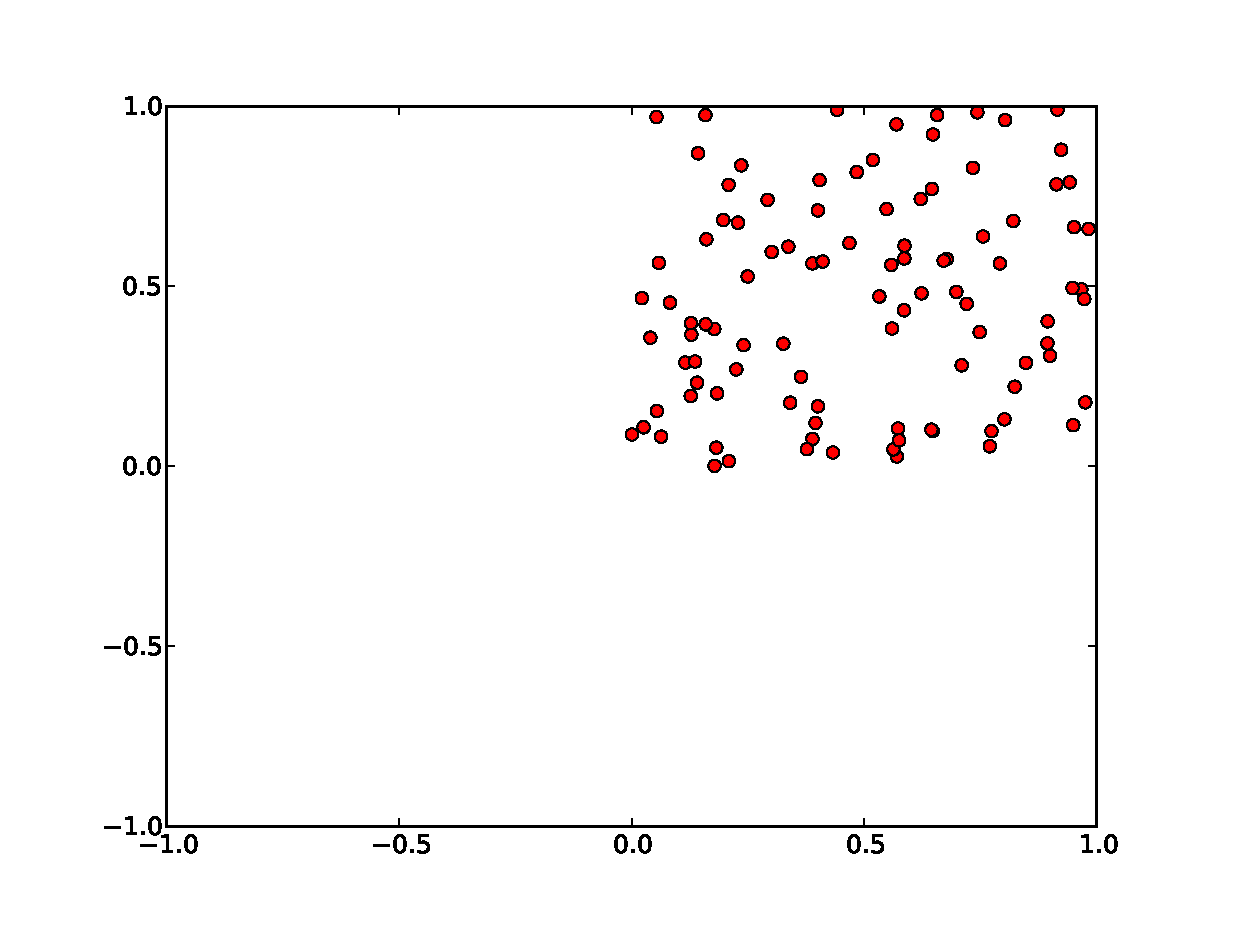
\includegraphics[width=0.47\textwidth]{images/coordinates_start.eps} \label{fig:firstbox}}
  \subfloat[]{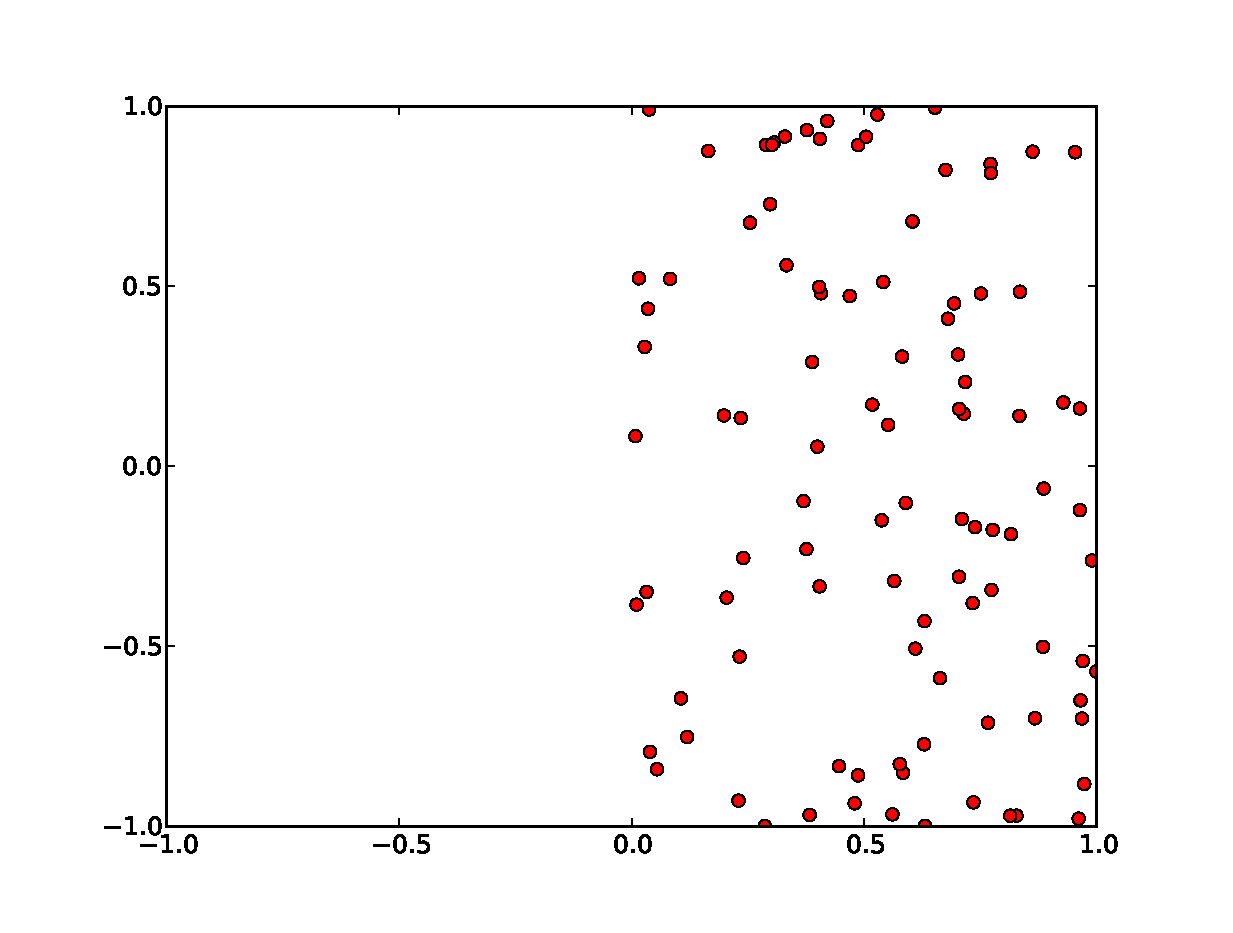
\includegraphics[width=0.47\textwidth]{images/coordinates_start_full.eps} \label{fig:secondbox}}
  \caption{
    Pyplot plot of particles in 2 dimensions confined in a box,
    spanning $x, y \in [0,1]$ for (a) and $y \in [-1,1]$ for (b).
  }
\end{figure}


\newpage

When you have corrected the particle positions, it is time to give the
particles random velocities to allow the particles to move around.

\begin{enumerate}
  \setcounter{enumi}{2}
  \item Create
    two new lists, \code{vel\_x} and \code{vel\_y}, which we shall use to
    store the velocities for the particles.
    The velocities should be a random number between -1 and 1.
\end{enumerate}

If you want to visualize the velocity vectors for each particle you can
use the following function.\\

\begin{lstlisting}
plt.quiver(pos_x, pos_y, vel_x, vel_y)
\end{lstlisting}

We are now ready to loop over each particle in our system, but before we do
this, you should make it really clear to yourself how we can obtain the
coordinates and velocities for the $i$'th particle.

\begin{enumerate}
  \setcounter{enumi}{3}
  \item How do we access the value of the $i$'th element in the \code{pos\_x} list?
      {\em Hint;} check out task (12) from part 1 again.

\end{enumerate}

In this weeks simulation there are no forces that acts on the particles,
and only their initial velocities influence their positions.
Hence the location of the $i$'th particle at time $n+1$ can be
calculated from the current time $n$'s coordinates and the velocity of the
particle.
\begin{align}
  x_i^{(n+1)} = x^n_i + v_{i}^n \cdot dt
\end{align}

That is, the $i$'th particle will be at its previous position plus its
velocity times a time step.

\begin{enumerate}
  \setcounter{enumi}{4}
  \item
    Modify your script to loop over each particle and update the $x$- and
    $y$-coordinates with the respective particle velocities.
    Plot the particle positions after you have changed them
    to a file called stepcoords.png. Does the particles appear to have have moved?

  \item Modify your code to repeat the displacement of the particles \code{n\_step} times.
      Remember to update the positions for each step.

  \item Where are the particles after 10 steps? 100 steps? 1000 steps? 10000 steps?
    Make a plot of the region (-1, 1, -1, 1) as well as (-10, 10, -10, 10) to
    help answer the question.

\end{enumerate}

What you simulate is how particles in vacuum behave if they can not feel
each other and have kinetic energy. What remains is to keep the particles
inside a box, i.e. they should make an elastic reflection on the walls and
change direction. \\

To change the direction on the $i$'th particle, we must change
the sign of the velocity for that particle. For simplicity, we shall add a box
which corresponds to the region we are plotting, that is $x \in [-1,1]$ 
and $y \in [-1,1]$.
We start out with the $x$-coordinates and then, when we
have confirmed that it is working, we move on to the $y$-coordinates.

\begin{enumerate}
  \setcounter{enumi}{7}
  \item Modify your code to check if the updated position of particle $i$ would violate $x \in [-1,1]$.
      If the particle is outside this boundary, change the sign of the $x$-velocity of that
      particular particle before the displacement is made.
      {\em Hint}; you will need if-statements to solve this problem. Also, it
      is a good idea to draw your plan for what happens with a pen and paper.

  \item Repeat for the $y$-direction.

\end{enumerate}

%\newpage

Now we would like to visualize the simulation we have made, because
it is a bit hard to see if the simulation has been implemented correctly by
just looking at a few images.
What we would like to do is to save a video of what we have done.
To make things easy (as any good cooking show), we have prepared
a method for you. \\

On the course website, there is a 'video.py' file.
Save this file, and put it in the same folder as the simulation file.
The function is implemented as following;

\begin{lstlisting}
import video

...

for n in range(n_steps):

    ...

    # Save a frame every 10 steps
    if n % 10 == 0:
        video.add_frame(pos_x, pos_y)

...

video.save('week1_video')

\end{lstlisting}

where the import statement should be positioned in the head of the file.
A video will be created called \code{week1\_video.mp4}

\begin{enumerate}
  \setcounter{enumi}{9}
  \item Run the simulation from task 9 for \code{n\_steps} = 1000 and save a video.
    Is the video of the simulation as you expect?

\end{enumerate}


% ***************************************************
% END DOCUMENT
% ***************************************************

\end{document}

